%% ------------------------------------------------------------------------- %%
\chapter{Introdução}
\label{cap:introducao}

SBC (Sociedade Brasileira de Computação)

“Discorrer sobre o tema escolhido e sobre o problema específico que você abordou, de forma que as pessoas que venham a ler esta introdução tenham uma ideia inicial do seu trabalho”. Sociedade Brasileira de Computação (SBC) sakdosaodksaokdsa daspdsa 

Este capítulo deve conter o objetivo do trabalho, qual é a principal contribuição do trabalho, os resultados importantes, e uma explicação de como os resultados foram obtidos. 

Pontos importantes a serem apresentados:
\begin{enumerate}[label={\alph*}]
    \item) lista numerada ou alpha
	\item) Tema de pesquisa;
	\item) Aspectos históricos (se houver);
	\item) Estado da arte (breve);
	\item) Contextualização
\end{enumerate}

SBC é a sociedade que coordena eventos científicos da computação no Brasil.

LEMBRAR DE FAZER CORRETAMENTE AS REFERÊNCIAS/CITAÇÕES. 
Exemplo de citação ~\cite{rabiner:1978}.

Exemplo de figura:
	
	\begin{figure}[!h]
	\centering
	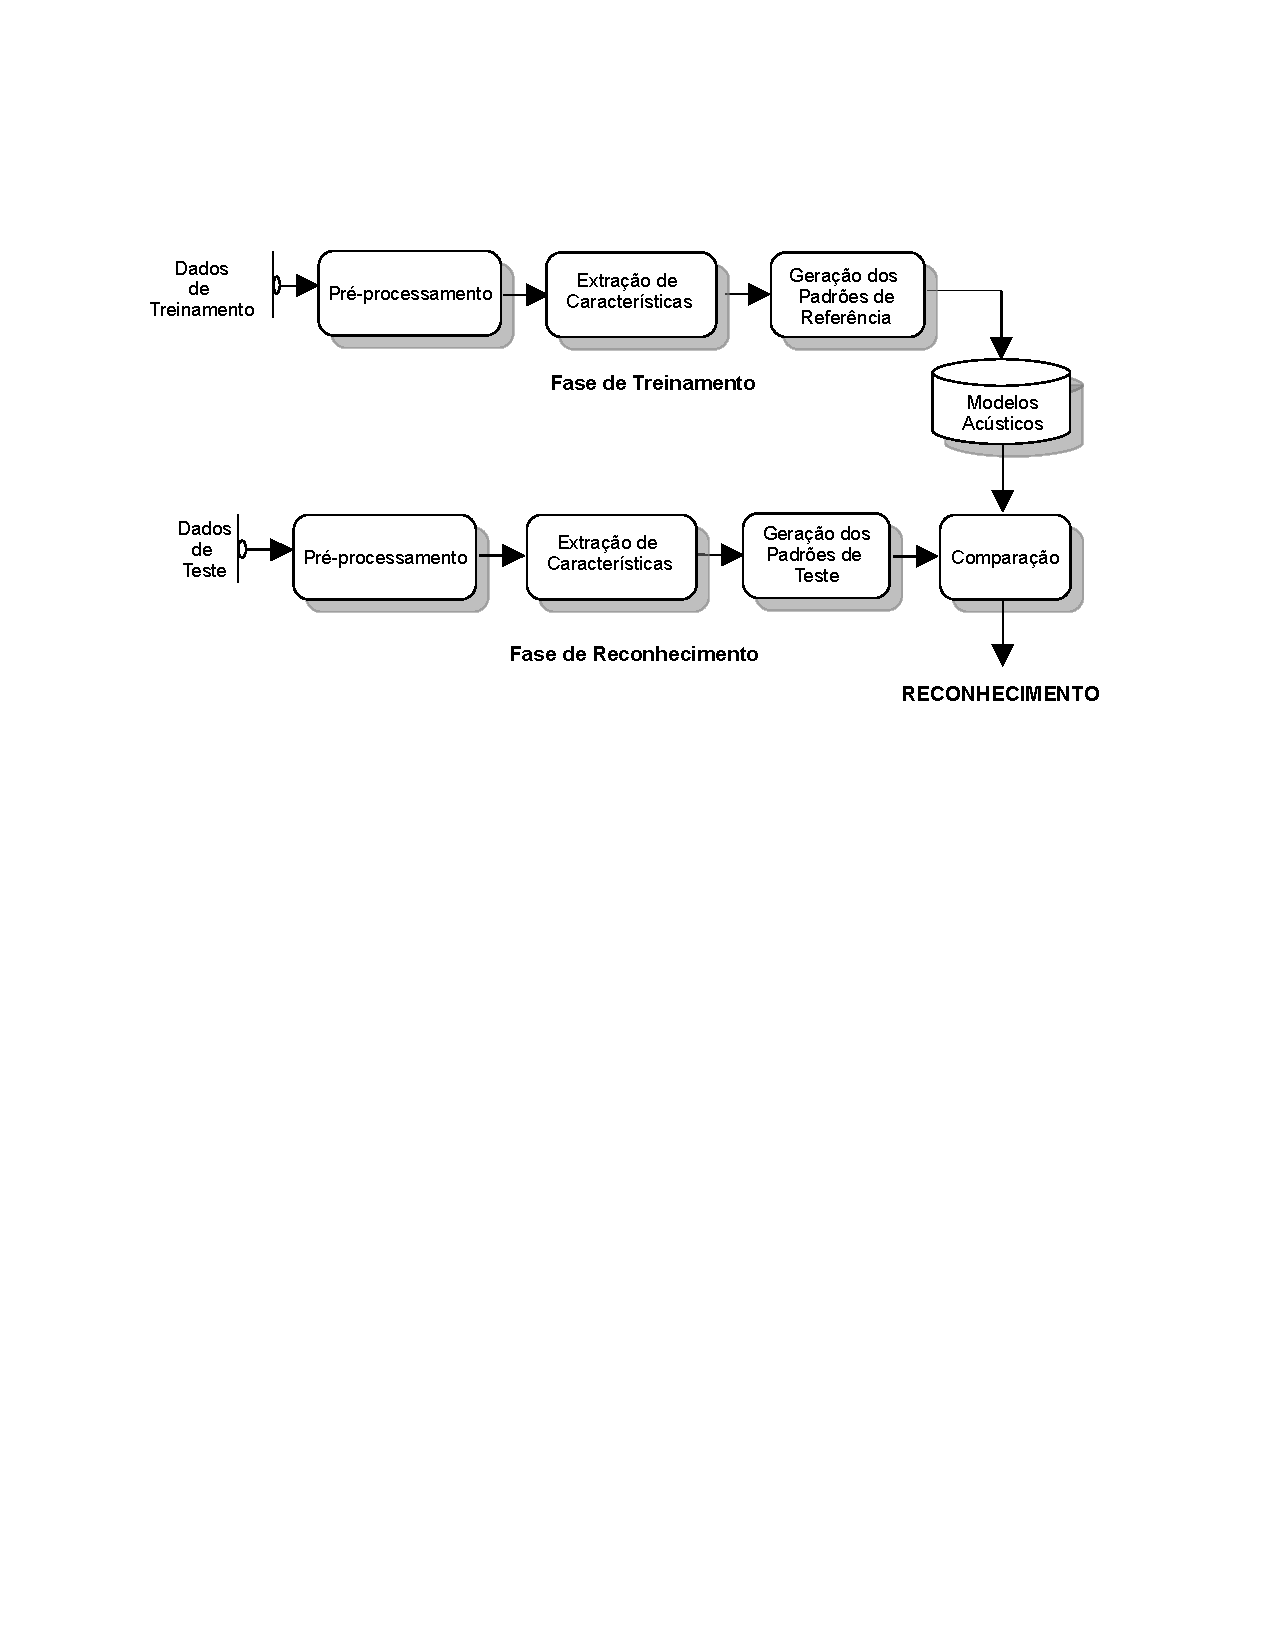
\includegraphics[width=.80\textwidth]{classificacao_padroes} 
	\caption{Sistema de reconhecimento de padrões aplicado ao reconhecimento de fala (Adaptada de ~\cite{rabiner:1978}.}
	\label{fig:class_padroes} 
	\end{figure}

\begin{figure}[!htpb]
    \centering
    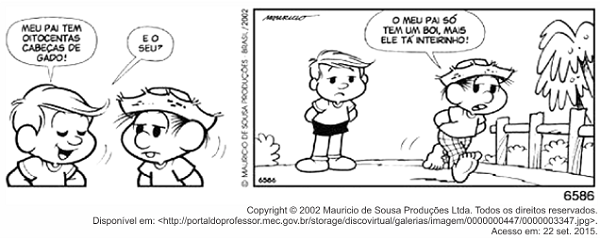
\includegraphics[width=1\textwidth]{minhasfigurasdotcc/metonimia.png}
    \caption{Exemplo de Figura}
    \label{fig:exemplo_de_figura}
\end{figure}


Um exemplo de tabela...\\

\underline{\textbf{Locutores masculinos}}
\begin{table}[htbp]
\centering 
\scalebox{0.7} {
	\begin{tabular}{ l | l | l | l | l | l }
	locutor&listas&faixa etária&profissão&escolaridade&Cidade/Estado\\ \hline
	\textbf{m01}&1 a 4&18 a 60 anos&estudante&superior&São Paulo - SP \\
	m02&5 a 8&18 a 60 anos&engenheiro&superior&Piracicaba – SP\\
	m03&13 a 16&18 a 60 anos&engenheiro&superior&Sta. B. D’Oeste - SP\\
	m04&17 a 20&18 a 60 anos&engenheiro&superior&Fortaleza - CE\\
	m05&9 a 12&18 a 60 anos&engenheiro&superior&S. Caetano do Sul - SP\\
	m06&13 a 16&18 a 60 anos&analista sist.&superior&Ribeirão Preto - SP\\
	m07&1 a 4&18 a 60 anos&professor&superior&São Carlos - SP\\
	m09&9 a 12&18 a 60 anos&estudante&superior&Limeira - SP\\
	\textbf{m11}&13 a 16&18 a 60 anos&estudante&superior&Tupã - SP\\
	m12&17 a 20&18 a 60 anos&estudante&superior&São Paulo – SP\\
	m13&17 a 20&18 a 60 anos&estudante&superior&Santos - SP\\
	m14&1 a 4&18 a 60 anos&comerciante&2o grau&Cotia - SP\\
	\textbf{m15}&17 a 20&18 a 60 anos&engenheiro&superior&Goiânia – GO\\
	m16&5 a 8&18 a 60 anos&estudante&superior&Bauru – SP\\
	\textbf{m17}&9 a 12&18 a 60 anos&estudante&superior&Porto Feliz - SP\\
	m18&5 a 8&18 a 60 anos&estudante&superior&Brasília - DF\\
	m20&1 a 4&18 a 60 anos&estudante&superior&São Paulo – SP\\
	m21&9 a 12&18 a 60 anos&estudante&superior&São Paulo - SP\\
	\textbf{m23}&5 a 8&18 a 60 anos&estudante&superior&Piracicaba - SP\\
	m24&13 a 16&18 a 60 anos&estudante&superior&S. Joaquim da Barra - SP\\
	\end{tabular}
}
\caption{Locutores masculinos utilizados na base de dados.}
\label{tab:locutoresmasculinos}
\end{table}


\begin{table}[!htpb]
    \centering
    \begin{tabular}{||l|c||}
       \hline
       \hline
        \textbf{Compra} &  \textbf{Valor}\\
        \hline
        \hline
         Supermercado & R\$ 250,00  \\
         \hline
         Combustível & R\$ 400,00 \\
         Escola & R\$ 750,00\\
         Inglês & R\$ 250,00\\
         \hline
         Academia & R\$ 60,00\\
         \hline
         \hline
    \end{tabular}
    \caption{Meu Exemplo de Tabela}
    \label{tab:my_label}
\end{table}

asdsad $x = y + z$ asdasdasdas

\begin{equation}
    a^2 = b^2 + c^2
    \label{eq:pitagoras}
\end{equation}

\begin{equation}
    \int_0^{2\pi} \int_{x-78}^{x} f(x, y)\; dydx
\end{equation}

\begin{equation}
    x = \frac{-b\pm \sqrt{b^2-4ac}}{2a}
    \label{eq:baskara}
\end{equation}

asidasdjsaidasdjia sdksaodoadokso, conforme visto na equação \ref{eq:baskara}, existe a necessidade de calcular tanto os pontos localizados na área positiva e negativa do plano do cartesiano.

%% ------------------------------------------------------------------------- %%
\section{Justificativa e Relevância do Trabalho}
\label{sec:justificativa}

Explicar porque foi escolhido esse tema, qual sua importância para a área, etc...


%% ------------------------------------------------------------------------- %%
\section{Objetivos}
\label{sec:objetivo}

\subsection{Objetivo Geral}
\label{sec:objgeral}
	O objetivo principal deste trabalho ......


\subsection{Objetivos Específicos}
\label{sec:objespecificos}

	\begin{itemize}
		\item XXXXXXXXXX
	
		\item XXXXXXXXXXX
	
	\end{itemize}



%% ------------------------------------------------------------------------- %%
\section{Metodologia}
\label{sec:metodologia}

A metodologia empregada para desenvolvimento do trabalho ...........\\


%% ------------------------------------------------------------------------- %%
\section{Organização do Documento}
\label{sec:organizacao}

No Capítulo~\ref{cap:modelagem}, são apresentados os conceitos relacionados .........

No Apêndice \ref{ape:base}, é apresentada a base de dados utilizada no trabalho.....
